\documentclass[12pt]{article}
\usepackage{xcolor}
\pagecolor{brown!20}
\usepackage{tikz}
\usetikzlibrary{positioning}
\usetikzlibrary{fit}
\usetikzlibrary{arrows.meta}
\usepackage{braket}%for \set command

\usepackage{fontspec}
\setmainfont{Liberation Serif}

\newcommand\lmaxsize{35}
\newcommand\lmaxsizeb{72}



%-----------------------------------------
\begin{document}

\noindent\begin{tikzpicture}[x=0.4cm,y=0.4cm]
\draw[blue!20, very thin] (1,1) grid (\lmaxsize,\lmaxsize);

\foreach \x in {1,...,\lmaxsize}{%
\node[circle,fill=yellow!40!green!30] at (\x,1) {ѻ};
}
%\node at (2,1) {ѻ};
%\node at (3,1) {ѻ};
%\node at (4,1) {ѻ};

\foreach \x in {1,...,\lmaxsize}{%
\node[circle,fill=blue] (n\x) at (\x,\x) {};%ѻ
}

\foreach \x in {6,12,18,30}{%
\node[pin=120:$\x$]  at (\x,\x) {};%ѻ
}
%\node[pin=120:$12$] at (12,12) {};
\node[draw=red,circle,thick,fit=(n8)(n9)(n10),label=above left:\textcolor{red}{$3$},inner sep=0pt] {};
\node[draw=red,circle,thick,fit=(n14)(n15)(n16),label=above left:\textcolor{red}{$3$},inner sep=0pt] {};
\node[draw=red,circle,thick,fit=(n20)(n21)(n22),label=above left:\textcolor{red}{$3$},inner sep=0pt] {};
\node[draw=red,circle,thick,fit=(n24)(n25)(n26)(n27)(n28),label=above left:\textcolor{red}{$5$},inner sep=0pt] {};


\foreach \x in {1,...,17}{%
\node[circle,fill=red] at (2*\x,\x) {};%ѻ
}

\foreach \x in {1,...,12}{%
\node[circle,fill=red!30!yellow] at (3*\x,\x) {};%ѻ
}

\foreach \x in {1,...,9}{%
\node[circle,fill=green!30!cyan] at (4*\x,\x) {};%ѻ
}

\foreach \x in {1,...,7}{%
\node[circle,fill=brown] at (5*\x,\x) {};%ѻ
}

\foreach \x in {1,...,2}{%
\node[circle,fill=violet] at (6*\x,\x) {};%ѻ
}

%primes
%3
\draw[fill=cyan] (2.9,1.2) rectangle (3.1,2.8);
%5
\draw[fill=cyan] (4.9,1.2) rectangle (5.1,4.8);
%7
\draw[fill=cyan] (6.9,1.2) rectangle (7.1,6.8);
%11
\draw[fill=cyan] (10.9,1.2) rectangle (11.1,10.8);
%13
\draw[fill=cyan] (12.9,1.2) rectangle (13.1,12.8);
%17
\draw[fill=cyan] (16.9,1.2) rectangle (17.1,16.8);
%19
\draw[fill=cyan] (18.9,1.2) rectangle (19.1,18.8);
%23
\draw[fill=cyan] (22.9,1.2) rectangle (23.1,22.8);
%29
\draw[fill=cyan] (28.9,1.2) rectangle (29.1,28.8);
%31
\draw[fill=cyan] (30.9,1.2) rectangle (31.1,30.8);

%orthogonal
\draw[->,very thick] (3,3) -- (6,0);%(5,1);
\draw[->,very thick, blue, dashed] (6,6) -- (6,0);%(6,1);
%parallel
\draw[->,very thick] (35,29) -- (6,0);%(7,1);


\draw[->,very thick] (6,6) -- (12,0);%(11,1);
\draw[->,very thick, blue, dashed] (12,12) -- (12,0);%(12,1);
\draw[->,very thick] (35,23) -- (12,0);%(13,1);

\draw[->,very thick, blue, dashed] (18,18) -- (18,0);%(12,1);
\draw[->,very thick, blue, dashed] (30,30) -- (30,0);%(12,1);



\node at (1,-0.5) {0};
\node at (2,-0.5) {0};
\node at (3,-0.5) {0};
\node at (4,-0.5) {1};
\node at (5,-0.5) {0};
\node at (6,-0.5) [rectangle,fill=yellow] {2};
\node at (7,-0.5) {0};
\node at (8,-0.5) {2};
\node at (9,-0.5) {1};
\node at (10,-0.5) {2};
\node at (11,-0.5) {0};
\node at (12,-0.5)[rectangle,fill=yellow] {4};
\node at (13,-0.5) {0};
\node at (14,-0.5) {1};
\node at (15,-0.5) {2};
\node at (16,-0.5) {2};
\node at (17,-0.5) {0};
\node at (18,-0.5) [rectangle,fill=yellow] {2};
\node at (19,-0.5) {0};
\node at (20,-0.5) {3};
\node at (21,-0.5) {1};
\node at (22,-0.5) {1};
\node at (23,-0.5) {0};
\node at (24,-0.5) {3};
\node at (25,-0.5) {1};
\node at (26,-0.5) {1};
\node at (27,-0.5) {1};
\node at (28,-0.5) {2};
\node at (29,-0.5) {0};
\node at (30,-0.5) [rectangle,fill=yellow] {3};
\node at (31,-0.5) {0};



\end{tikzpicture}


\newpage

\noindent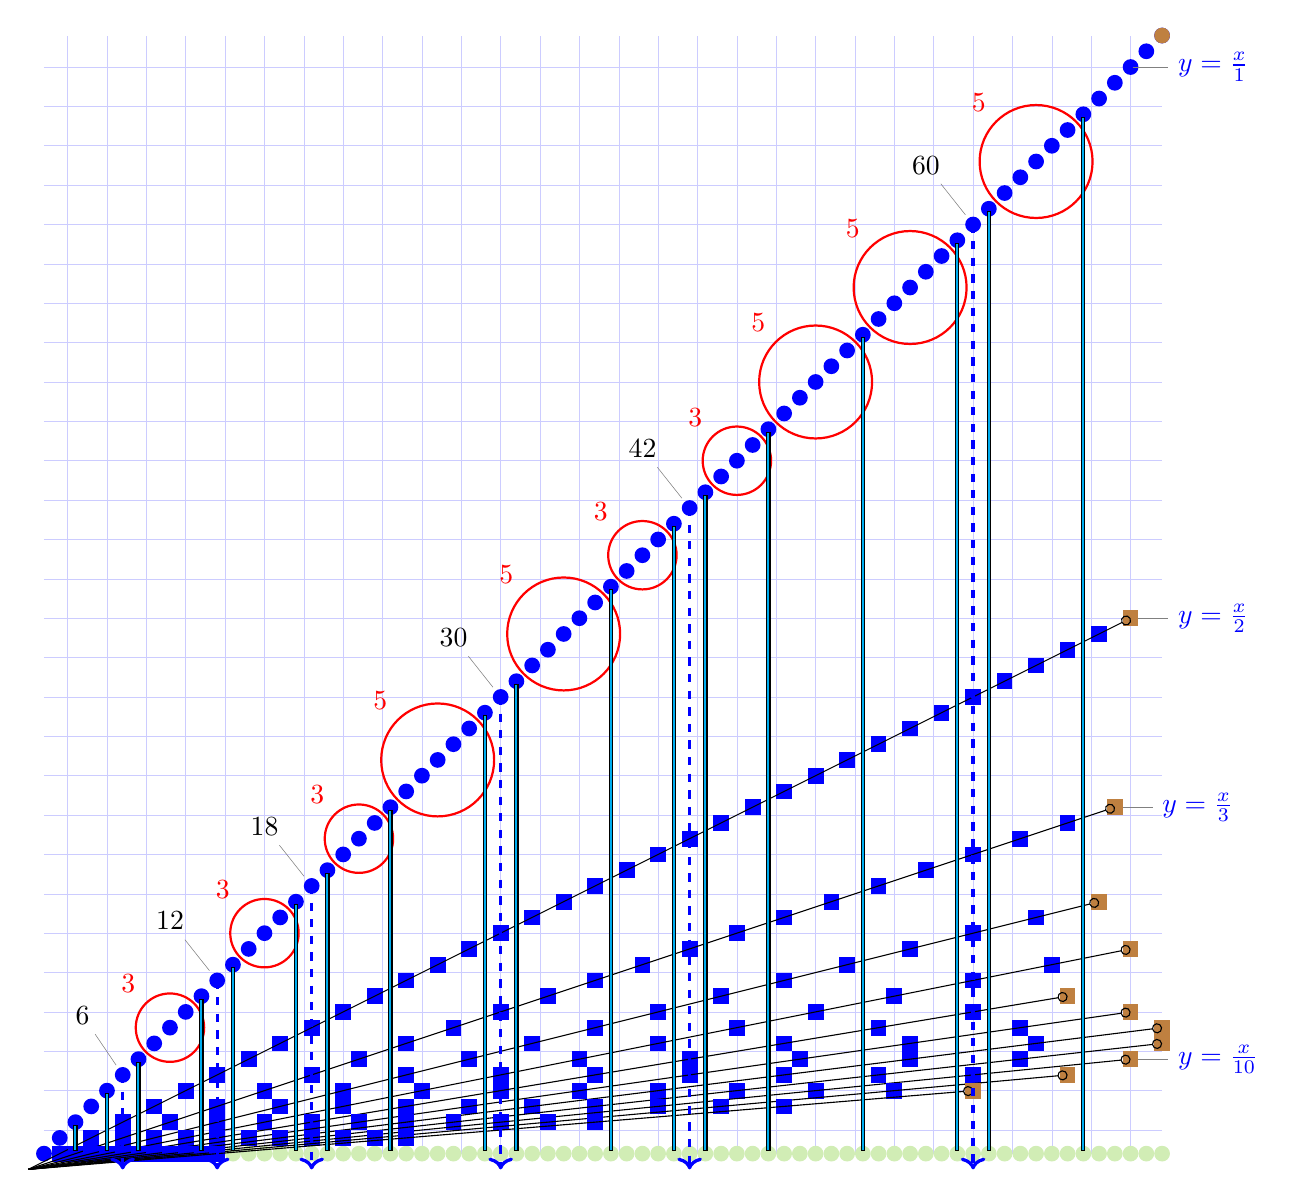
\begin{tikzpicture}[x=0.4cm,y=0.4cm,scale=0.5]
\draw[blue!20, very thin] (1,1) grid (\lmaxsizeb,\lmaxsizeb);

\foreach \x in {1,...,\lmaxsizeb}{%
\node[circle,
inner sep=0pt,
minimum size=2mm,
fill=yellow!40!green!30] at (\x,1) {};%ѻ
}
%\node at (2,1) {ѻ};
%\node at (3,1) {ѻ};
%\node at (4,1) {ѻ};

\foreach \x in {1,...,\lmaxsizeb}{%
\node[circle,
inner sep=0pt,
minimum size=2mm,
fill=blue] (n\x) at (\x,\x) {};%ѻ
}
%last one:
\node[circle,
inner sep=0pt,
minimum size=2mm,fill=brown] at (\lmaxsizeb,\lmaxsizeb) {};%ѻ



\foreach \x in {6,12,18,30,42,60}{%
\node[pin=120:$\x$]  at (\x,\x) {};%ѻ
}
\node[pin={[blue]right:$y=\frac{x}{1}$},inner sep=0pt] at (70,70) {};

%non-primes
%\node[pin=120:$12$] at (12,12) {};
\node[draw=red,circle,thick,fit=(n8)(n9)(n10),label=above left:\textcolor{red}{$3$},inner sep=0pt] {};
\node[draw=red,circle,thick,fit=(n14)(n15)(n16),label=above left:\textcolor{red}{$3$},inner sep=0pt] {};
\node[draw=red,circle,thick,fit=(n20)(n21)(n22),label=above left:\textcolor{red}{$3$},inner sep=0pt] {};
\node[draw=red,circle,thick,fit=(n24)(n25)(n26)(n27)(n28),label=above left:\textcolor{red}{$5$},inner sep=0pt] {};
\node[draw=red,circle,thick,fit=(n32)(n33)(n34)(n35)(n36),label=above left:\textcolor{red}{$5$},inner sep=0pt] {};
\node[draw=red,circle,thick,fit=(n38)(n39)(n40),label=above left:\textcolor{red}{$3$},inner sep=0pt] {};
\node[draw=red,circle,thick,fit=(n44)(n45)(n46),label=above left:\textcolor{red}{$3$},inner sep=0pt] {};
\node[draw=red,circle,thick,fit=(n48)(n49)(n50)(n51)(n52),label=above left:\textcolor{red}{$5$},inner sep=0pt] {};
\node[draw=red,circle,thick,fit=(n54)(n55)(n56)(n57)(n58),label=above left:\textcolor{red}{$5$},inner sep=0pt] {};
\node[draw=red,circle,thick,fit=(n62)(n63)(n64)(n65)(n66),label=above left:\textcolor{red}{$5$},inner sep=0pt] {};



%----------2
\foreach \x in {1,...,35}{%
\node[
inner sep=0pt,
minimum size=2mm,fill=blue] at (2*\x,\x) {};%ѻ
}
\node[pin={[blue]right:$y=\frac{x}{2}$},inner sep=0pt] at (70,35) {};
%last one:
\node[
inner sep=0pt,
minimum size=2mm,fill=brown] at (70,35) {};%ѻ
%line:
\draw[-{Circle[open]}] (0,0) -- (70,35);



%----------3
\foreach \x in {1,...,23}{%
\node[
inner sep=0pt,
minimum size=2mm,fill=blue] at (3*\x,\x) {};%ѻ
}
\node[pin={[blue]right:$y=\frac{x}{3}$},inner sep=0pt] at (69,23) {};
%last one:
\node[
inner sep=0pt,
minimum size=2mm,fill=brown] at (69,23) {};%ѻ
%line:
\draw[-{Circle[open]}] (0,0) -- (69,23);



%----------4
\foreach \x in {1,...,17}{%
\node[
inner sep=0pt,
minimum size=2mm,fill=blue] at (4*\x,\x) {};%ѻ
}
%last one:
\node[
inner sep=0pt,
minimum size=2mm,fill=brown] at (68,17) {};%ѻ
%line:
\draw[-{Circle[open]}] (0,0) -- (68,17);



%----------5
\foreach \x in {1,...,14}{%
\node[
inner sep=0pt,
minimum size=2mm,fill=blue] at (5*\x,\x) {};%ѻ
}
%last one:
\node[
inner sep=0pt,
minimum size=2mm,fill=brown] at (70,14) {};%ѻ
%line:
\draw[-{Circle[open]}] (0,0) -- (70,14);



%----------6
\foreach \x in {1,...,11}{%
\node[
inner sep=0pt,
minimum size=2mm,fill=blue] at (6*\x,\x) {};%ѻ
}
%last one:
\node[
inner sep=0pt,
minimum size=2mm,fill=brown] at (66,11) {};%ѻ
%line:
\draw[-{Circle[open]}] (0,0) -- (66,11);



%----------7
\foreach \x in {1,...,10}{%
\node[
inner sep=0pt,
minimum size=2mm,fill=blue] at (7*\x,\x) {};%ѻ
}
%last one:
\node[
inner sep=0pt,
minimum size=2mm,fill=brown] at (70,10) {};%ѻ
%line:
\draw[-{Circle[open]}] (0,0) -- (70,10);



%----------8
\foreach \x in {1,...,9}{%
\node[
inner sep=0pt,
minimum size=2mm,fill=blue] at (8*\x,\x) {};%ѻ
}
%last one:
\node[
inner sep=0pt,
minimum size=2mm,fill=brown] at (72,9) {};%ѻ
%line:
\draw[-{Circle[open]}] (0,0) -- (72,9);



%----------9
\foreach \x in {1,...,8}{%
\node[
inner sep=0pt,
minimum size=2mm,fill=blue] at (9*\x,\x) {};%ѻ
}
%last one:
\node[
inner sep=0pt,
minimum size=2mm,fill=brown] at (72,8) {};%ѻ
%line:
\draw[-{Circle[open]}] (0,0) -- (72,8);



%----------10
\foreach \x in {1,...,7}{%
\node[
inner sep=0pt,
minimum size=2mm,fill=blue] at (10*\x,\x) {};%ѻ
}
\node[pin={[blue]right:$y=\frac{x}{10}$},inner sep=0pt] at (70,7) {};
%last one:
\node[
inner sep=0pt,
minimum size=2mm,fill=brown] at (70,7) {};%ѻ
%line:
\draw[-{Circle[open]}] (0,0) -- (70,7);



%----------11
\foreach \x in {1,...,6}{%
\node[
inner sep=0pt,
minimum size=2mm,fill=blue] at (11*\x,\x) {};%ѻ
}
%last one:
\node[
inner sep=0pt,
minimum size=2mm,fill=brown] at (66,6) {};%ѻ
%line:
\draw[-{Circle[open]}] (0,0) -- (66,6);



%----------12
\foreach \x in {1,...,5}{%
\node[
inner sep=0pt,
minimum size=2mm,fill=blue] at (12*\x,\x) {};%ѻ
}
%last one:
\node[
inner sep=0pt,
minimum size=2mm,fill=brown] at (60,5) {};%ѻ
%line:
\draw[-{Circle[open]}] (0,0) -- (60,5);



%primes
\foreach \x in {3,5,7,11, 13, 17, 19, 23, 29, 31, 37, 41, 43, 47, 53, 59, 61, 67}{%
\draw[fill=cyan] (\x-0.1,1.2) rectangle (\x+0.1,\x-0.2);
}
%3
%\draw[fill=cyan] (2.9,1.2) rectangle (3.1,2.8);
%%5
%\draw[fill=cyan] (4.9,1.2) rectangle (5.1,4.8);
%%7
%\draw[fill=cyan] (6.9,1.2) rectangle (7.1,6.8);
%%11
%\draw[fill=cyan] (10.9,1.2) rectangle (11.1,10.8);
%%13
%\draw[fill=cyan] (12.9,1.2) rectangle (13.1,12.8);
%%17
%\draw[fill=cyan] (16.9,1.2) rectangle (17.1,16.8);
%%19
%\draw[fill=cyan] (18.9,1.2) rectangle (19.1,18.8);
%%23
%\draw[fill=cyan] (22.9,1.2) rectangle (23.1,22.8);
%%29
%\draw[fill=cyan] (28.9,1.2) rectangle (29.1,28.8);
%%31
%\draw[fill=cyan] (30.9,1.2) rectangle (31.1,30.8);
%%37
%\draw[fill=cyan] (36.9,1.2) rectangle (37.1,36.8);
%%41
%\draw[fill=cyan] (40.9,1.2) rectangle (41.1,40.8);
%%43
%\draw[fill=cyan] (42.9,1.2) rectangle (43.1,42.8);
%%47
%\draw[fill=cyan] (47-0.1,1.2) rectangle (47+0.1,47-0.2);
%%53
%\draw[fill=cyan] (53-0.1,1.2) rectangle (53+0.1,53-0.2);
%%59
%\draw[fill=cyan] (47-0.1,1.2) rectangle (47+0.1,47-0.2);
%%61
%\draw[fill=cyan] (47-0.1,1.2) rectangle (47+0.1,47-0.2);
%%67
%\draw[fill=cyan] (47-0.1,1.2) rectangle (47+0.1,47-0.2);



%orthogonal
%\draw[->,very thick] (3,3) -- (6,0);%(5,1);
\draw[->,very thick, blue, dashed] (6,6) -- (6,0);%(6,1);
%parallel
%\draw[->,very thick] (35,29) -- (6,0);%(7,1);


%\draw[->,very thick] (6,6) -- (12,0);%(11,1);
\draw[->,very thick, blue, dashed] (12,12) -- (12,0);%(12,1);
%\draw[->,very thick] (35,23) -- (12,0);%(13,1);

\draw[->,very thick, blue, dashed] (18,18) -- (18,0);%(12,1);
\draw[->,very thick, blue, dashed] (30,30) -- (30,0);%(12,1);
\draw[->,very thick, blue, dashed] (42,42) -- (42,0);%(12,1);
\draw[->,very thick, blue, dashed] (60,60) -- (60,0);%(12,1);


%Here are the first few prime numbers: 2, 3, 5, 7, 11, 13, 17, 19, 23, 29, 31, 37, 41, 43, 47, 53, 59, 61, 67, 71, 73, 79, 83, 89, 97, 101, 103, 107, 109, 113, 127, 131, 137, 139, 149, 151, 157, 163, 167, 173, 179, 181, 191, 193, 197, 199, etc.


%\node at (1,-0.5) {0};
%\node at (2,-0.5) {0};
%\node at (3,-0.5) {0};
%\node at (4,-0.5) {1};
%\node at (5,-0.5) {0};
%\node at (6,-0.5) [rectangle,fill=yellow] {2};
%\node at (7,-0.5) {0};
%\node at (8,-0.5) {2};
%\node at (9,-0.5) {1};
%\node at (10,-0.5) {2};
%\node at (11,-0.5) {0};
%\node at (12,-0.5)[rectangle,fill=yellow] {4};
%\node at (13,-0.5) {0};
%\node at (14,-0.5) {1};
%\node at (15,-0.5) {2};
%\node at (16,-0.5) {2};
%\node at (17,-0.5) {0};
%\node at (18,-0.5) [rectangle,fill=yellow] {2};
%\node at (19,-0.5) {0};
%\node at (20,-0.5) {3};
%\node at (21,-0.5) {1};
%\node at (22,-0.5) {1};
%\node at (23,-0.5) {0};
%\node at (24,-0.5) {3};
%\node at (25,-0.5) {1};
%\node at (26,-0.5) {1};
%\node at (27,-0.5) {1};
%\node at (28,-0.5) {2};
%\node at (29,-0.5) {0};
%\node at (30,-0.5) [rectangle,fill=yellow] {3};
%\node at (31,-0.5) {0};



\end{tikzpicture}








\newpage

\noindent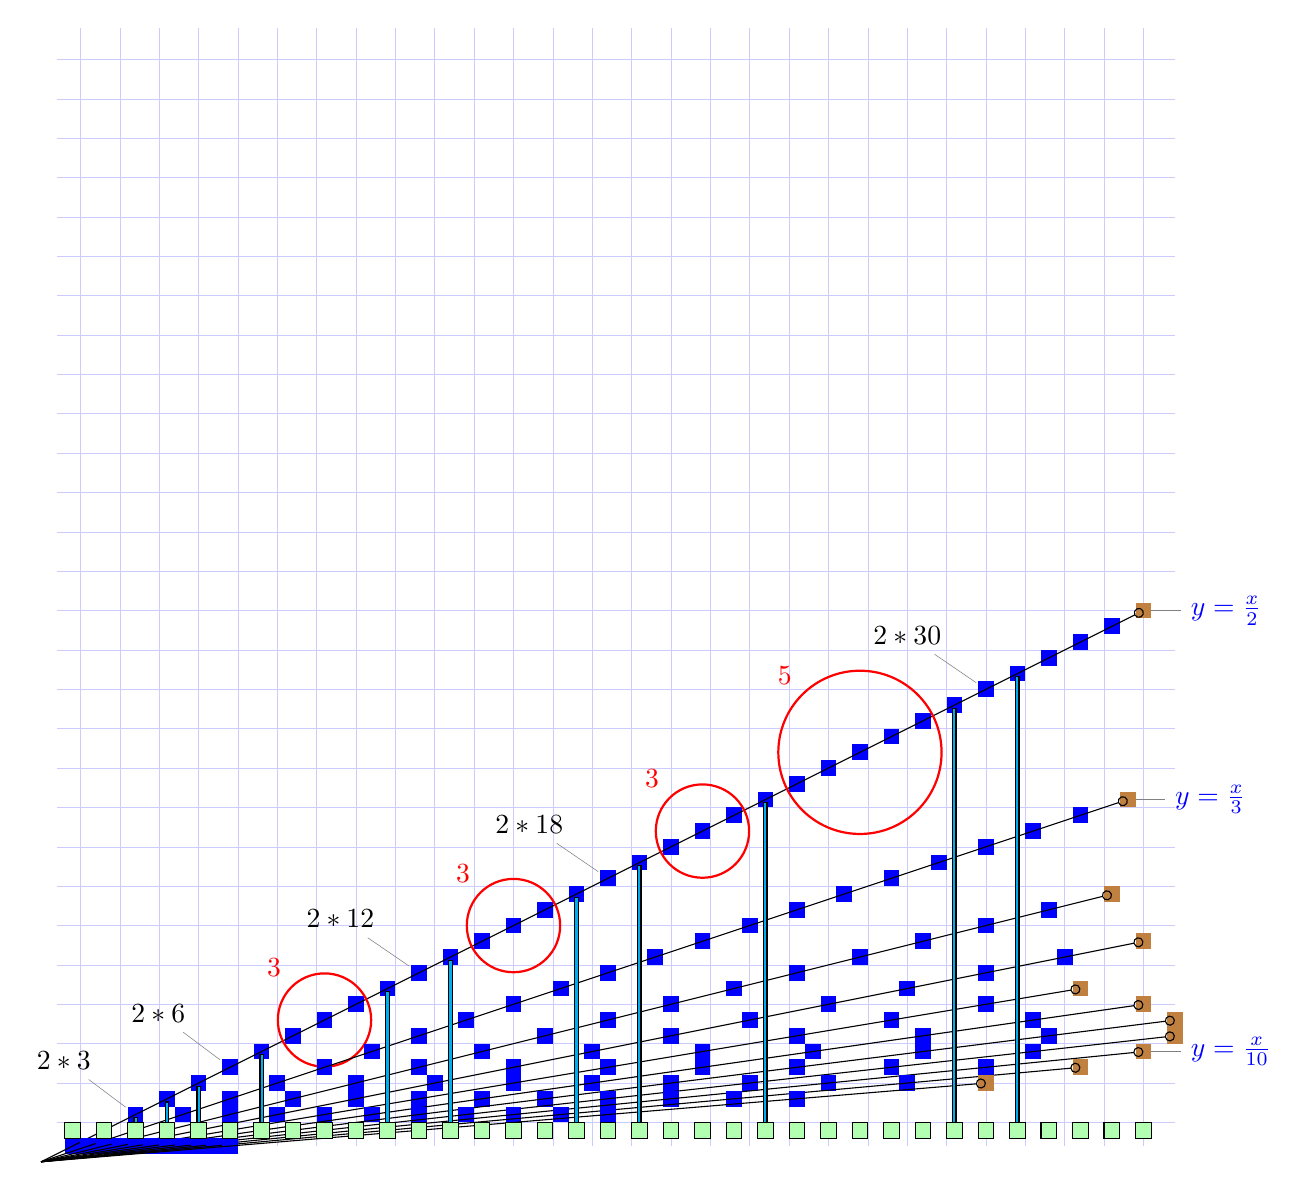
\begin{tikzpicture}[x=0.4cm,y=0.4cm,scale=0.5]
\draw[blue!20, very thin] (1,1) grid (\lmaxsizeb,\lmaxsizeb);


%\foreach \x in {1,...,\lmaxsizeb}{%
%\node[circle,
%inner sep=0pt,
%minimum size=2mm,
%fill=blue] (n\x) at (\x,\x) {};%ѻ
%}
%%last one:
%\node[circle,
%inner sep=0pt,
%minimum size=2mm,fill=brown] at (\lmaxsizeb,\lmaxsizeb) {};%ѻ



%\foreach \x in {6,12,18,30,42,60}{%
%\node[pin=120:$\x$]  at (\x,\x) {};%ѻ
%}
%\node[pin={[blue]right:$y=\frac{x}{1}$},inner sep=0pt] at (70,70) {};

%non-primes
%\node[draw=red,circle,thick,fit=(n8)(n9)(n10),label=above left:\textcolor{red}{$3$},inner sep=0pt] {};
%\node[draw=red,circle,thick,fit=(n14)(n15)(n16),label=above left:\textcolor{red}{$3$},inner sep=0pt] {};
%\node[draw=red,circle,thick,fit=(n20)(n21)(n22),label=above left:\textcolor{red}{$3$},inner sep=0pt] {};
%\node[draw=red,circle,thick,fit=(n24)(n25)(n26)(n27)(n28),label=above left:\textcolor{red}{$5$},inner sep=0pt] {};
%\node[draw=red,circle,thick,fit=(n32)(n33)(n34)(n35)(n36),label=above left:\textcolor{red}{$5$},inner sep=0pt] {};
%\node[draw=red,circle,thick,fit=(n38)(n39)(n40),label=above left:\textcolor{red}{$3$},inner sep=0pt] {};
%\node[draw=red,circle,thick,fit=(n44)(n45)(n46),label=above left:\textcolor{red}{$3$},inner sep=0pt] {};
%\node[draw=red,circle,thick,fit=(n48)(n49)(n50)(n51)(n52),label=above left:\textcolor{red}{$5$},inner sep=0pt] {};
%\node[draw=red,circle,thick,fit=(n54)(n55)(n56)(n57)(n58),label=above left:\textcolor{red}{$5$},inner sep=0pt] {};
%\node[draw=red,circle,thick,fit=(n62)(n63)(n64)(n65)(n66),label=above left:\textcolor{red}{$5$},inner sep=0pt] {};



%----------2
\foreach \x in {1,...,35}{%
\node[
inner sep=0pt,
minimum size=2mm,fill=blue] (n\x) at (2*\x,\x) {};%ѻ
}
\node[pin={[blue]right:$y=\frac{x}{2}$},inner sep=0pt] at (70,35) {};
%last one:
\node[
inner sep=0pt,
minimum size=2mm,fill=brown] at (70,35) {};%ѻ
%line:
\draw[-{Circle[open]}] (0,0) -- (70,35);
\node[draw=red,circle,thick,fit=(n8)(n9)(n10),label=above left:\textcolor{red}{$3$},inner sep=0pt] {};
\node[draw=red,circle,thick,fit=(n14)(n15)(n16),label=above left:\textcolor{red}{$3$},inner sep=0pt] {};
\node[draw=red,circle,thick,fit=(n20)(n21)(n22),label=above left:\textcolor{red}{$3$},inner sep=0pt] {};
\node[draw=red,circle,thick,fit=(n24)(n25)(n26)(n27)(n28),label=above left:\textcolor{red}{$5$},inner sep=0pt] {};



%----------3
\foreach \x in {1,...,23}{%
\node[
inner sep=0pt,
minimum size=2mm,fill=blue] at (3*\x,\x) {};%ѻ
}
\node[pin={[blue]right:$y=\frac{x}{3}$},inner sep=0pt] at (69,23) {};
%last one:
\node[
inner sep=0pt,
minimum size=2mm,fill=brown] at (69,23) {};%ѻ
%line:
\draw[-{Circle[open]}] (0,0) -- (69,23);



%----------4
\foreach \x in {1,...,17}{%
\node[
inner sep=0pt,
minimum size=2mm,fill=blue] at (4*\x,\x) {};%ѻ
}
%last one:
\node[
inner sep=0pt,
minimum size=2mm,fill=brown] at (68,17) {};%ѻ
%line:
\draw[-{Circle[open]}] (0,0) -- (68,17);



%----------5
\foreach \x in {1,...,14}{%
\node[
inner sep=0pt,
minimum size=2mm,fill=blue] at (5*\x,\x) {};%ѻ
}
%last one:
\node[
inner sep=0pt,
minimum size=2mm,fill=brown] at (70,14) {};%ѻ
%line:
\draw[-{Circle[open]}] (0,0) -- (70,14);



%----------6
\foreach \x in {1,...,11}{%
\node[
inner sep=0pt,
minimum size=2mm,fill=blue] at (6*\x,\x) {};%ѻ
}
%last one:
\node[
inner sep=0pt,
minimum size=2mm,fill=brown] at (66,11) {};%ѻ
%line:
\draw[-{Circle[open]}] (0,0) -- (66,11);



%----------7
\foreach \x in {1,...,10}{%
\node[
inner sep=0pt,
minimum size=2mm,fill=blue] at (7*\x,\x) {};%ѻ
}
%last one:
\node[
inner sep=0pt,
minimum size=2mm,fill=brown] at (70,10) {};%ѻ
%line:
\draw[-{Circle[open]}] (0,0) -- (70,10);



%----------8
\foreach \x in {1,...,9}{%
\node[
inner sep=0pt,
minimum size=2mm,fill=blue] at (8*\x,\x) {};%ѻ
}
%last one:
\node[
inner sep=0pt,
minimum size=2mm,fill=brown] at (72,9) {};%ѻ
%line:
\draw[-{Circle[open]}] (0,0) -- (72,9);



%----------9
\foreach \x in {1,...,8}{%
\node[
inner sep=0pt,
minimum size=2mm,fill=blue] at (9*\x,\x) {};%ѻ
}
%last one:
\node[
inner sep=0pt,
minimum size=2mm,fill=brown] at (72,8) {};%ѻ
%line:
\draw[-{Circle[open]}] (0,0) -- (72,8);



%----------10
\foreach \x in {1,...,7}{%
\node[
inner sep=0pt,
minimum size=2mm,fill=blue] at (10*\x,\x) {};%ѻ
}
\node[pin={[blue]right:$y=\frac{x}{10}$},inner sep=0pt] at (70,7) {};
%last one:
\node[
inner sep=0pt,
minimum size=2mm,fill=brown] at (70,7) {};%ѻ
%line:
\draw[-{Circle[open]}] (0,0) -- (70,7);



%----------11
\foreach \x in {1,...,6}{%
\node[
inner sep=0pt,
minimum size=2mm,fill=blue] at (11*\x,\x) {};%ѻ
}
%last one:
\node[
inner sep=0pt,
minimum size=2mm,fill=brown] at (66,6) {};%ѻ
%line:
\draw[-{Circle[open]}] (0,0) -- (66,6);



%----------12
\foreach \x in {1,...,5}{%
\node[
inner sep=0pt,
minimum size=2mm,fill=blue] at (12*\x,\x) {};%ѻ
}
%last one:
\node[
inner sep=0pt,
minimum size=2mm,fill=brown] at (60,5) {};%ѻ
%line:
\draw[-{Circle[open]}] (0,0) -- (60,5);



%2-primes
\foreach \x in {2,3,4,5,7,11, 13, 17, 19, 23, 29, 31}{%
\draw[fill=cyan] (2*\x-0.1,2.2) rectangle (2*\x+0.1,\x-0.2);
}



%orthogonal
\foreach \x in {3,6,12,18,30}{%
\node[pin=above left:$2*\x$] at (2*\x,\x) {};%ѻ
}

%\draw[->,very thick, blue, dashed] (6,6) -- (6,0);%(6,1);
%\draw[->,very thick, blue, dashed] (12,12) -- (12,0);%(12,1);
%\draw[->,very thick, blue, dashed] (18,18) -- (18,0);%(12,1);
%\draw[->,very thick, blue, dashed] (30,30) -- (30,0);%(12,1);
%\draw[->,very thick, blue, dashed] (42,42) -- (42,0);%(12,1);
%\draw[->,very thick, blue, dashed] (60,60) -- (60,0);%(12,1);



\foreach \x in {1,...,35}{%
\node[draw,
inner sep=0pt,
minimum size=2mm,
fill=green!30] at (2*\x,2) {};%ѻ
}

\end{tikzpicture}

$22$ and $26$ are primes in the $\mathit{2}$-prime set, because they are $2*11$ and $2*13$.

$p*12\pm p*1$, where the  prime-base $p \in \set{1,2,3,\ldots}$


\end{document}